\subsection{Toy Models}

The energy eigenstates and $\set{\ket{0},\ket{1}}$ coefficients for the $H \in \mathbb{R}^2$ Hamiltonian as a function of interaction strength $\lambda$ is shown in figure \cref{fig:res:changing_character}. Despite having two free parameters $C_0,C_1$ they are constrained through normalization.  
\begin{figure}[H]
    \centering
    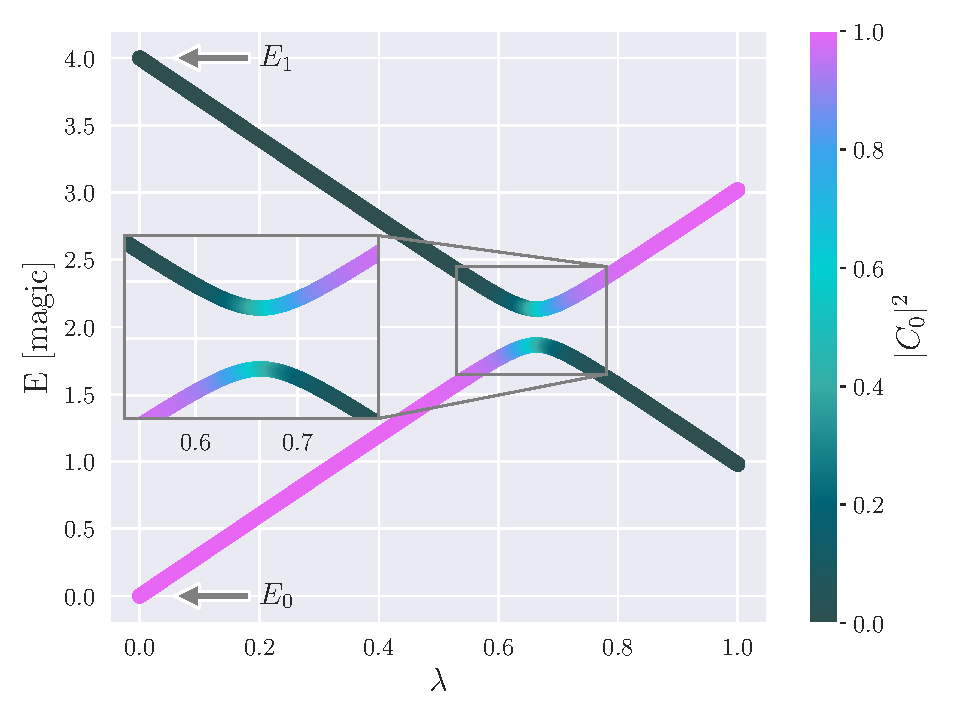
\includegraphics[width=\linewidth]{figs/chaning_character.pdf}
    \caption{Energy eigenstates and coefficients of $2 \times 2$ Hamiltonian when varying the interaction strength $\lambda \in [0,1]$. Calculations done using exact diagonalization.}
    \label[fig]{fig:res:changing_character}
\end{figure}

The entropy of entanglement in the case of the of the Hamiltonian consisting of a interacting and non-interacting between the two states, is presented in Fig. (\ref{fig:entropy}). It is apparent that the entropy of entanglement increases as the connection strength increases. 

\begin{figure}
    \centering
    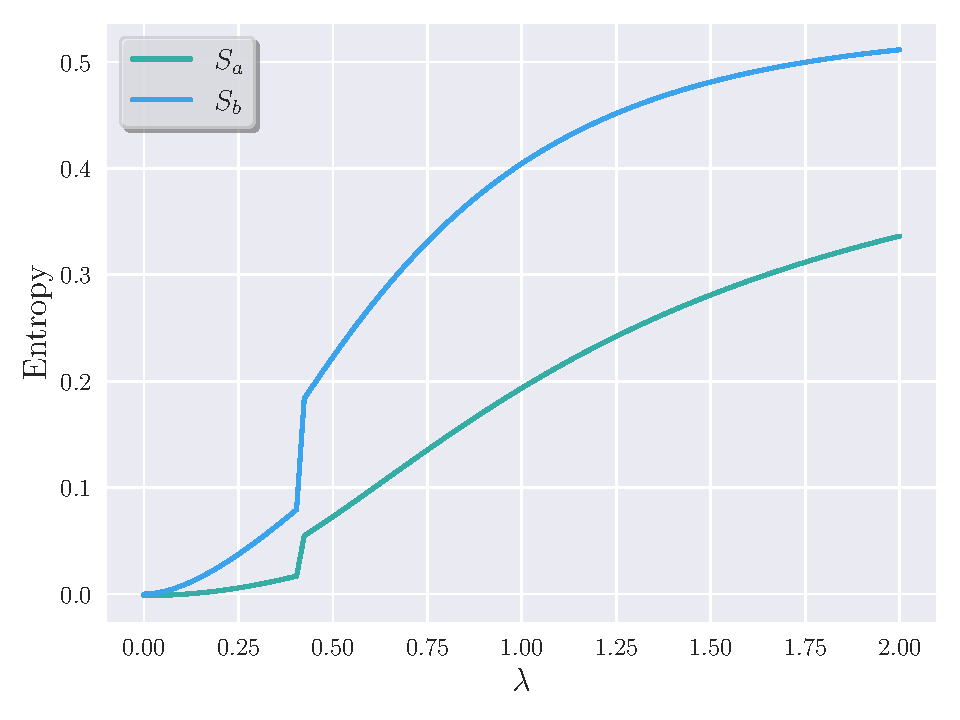
\includegraphics[scale=0.4]{figs/Entropy.pdf}
    \caption{Caption}
    \label{fig:entropy}
\end{figure}

\subsection{Lipkin Model}

\begin{figure}[H]
    \centering
    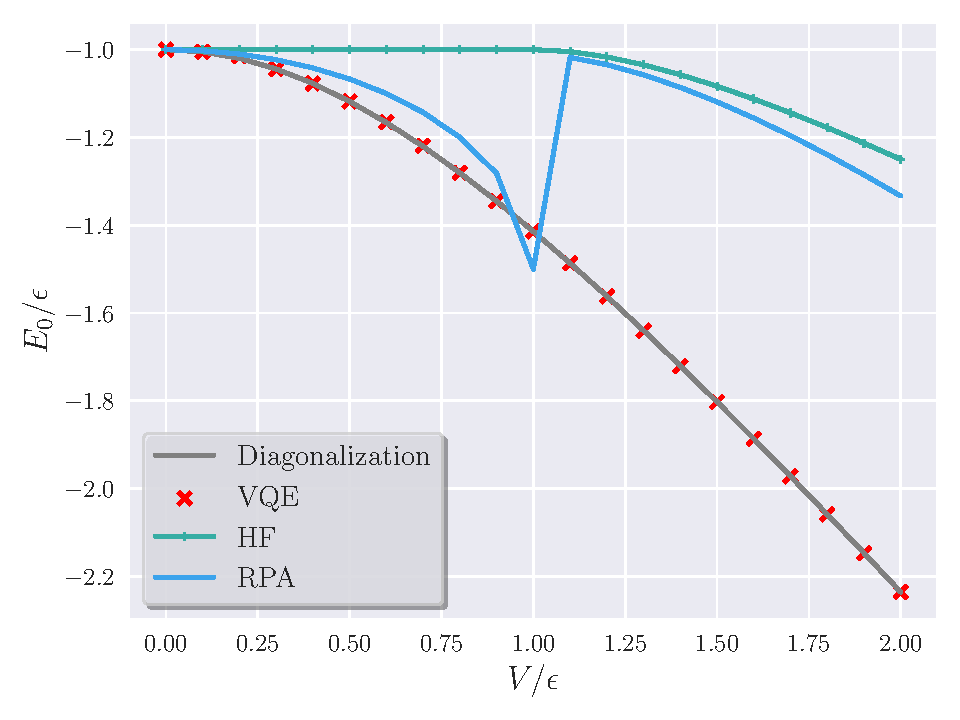
\includegraphics[width=\linewidth]{figs/N2_lipkin_vary_V.pdf}
    \caption{Ground state values for the Lipkin model for $N=2$ particles with $W = 0$ as a function of $V/\epsilon$. Calculations were done using exact diagonalization, VQE, in addition to closed form HF and RPA expressions.}
    \label[fig]{fig:res:Lipkin_N2_vary_v}
\end{figure}

\begin{figure}[H]
    \centering
    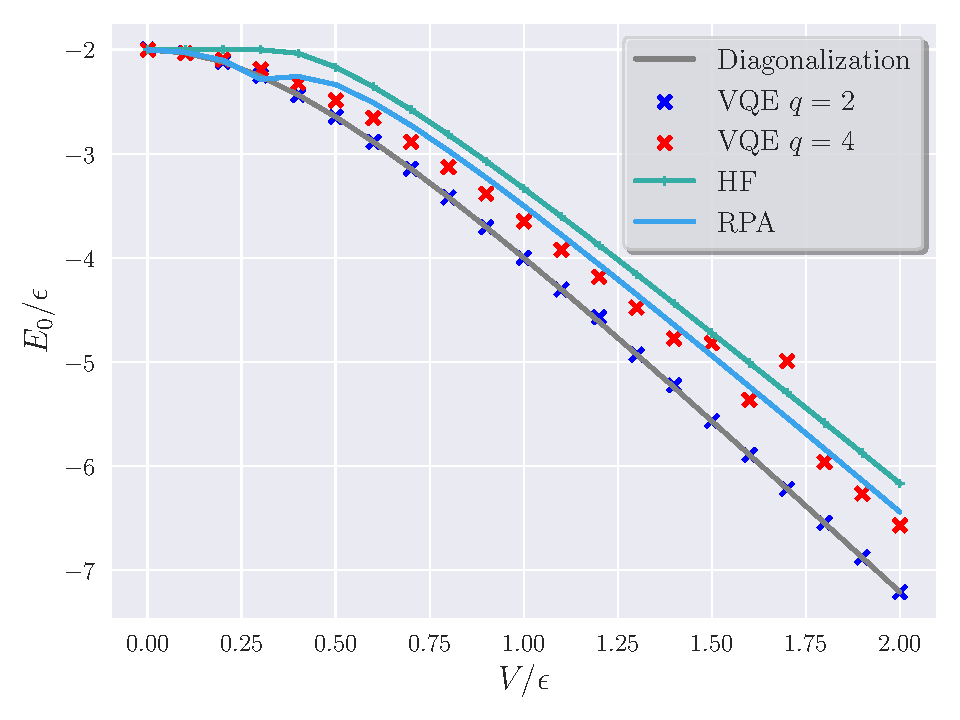
\includegraphics[width=\linewidth]{figs/N4_lipkin_vary_V.pdf}
    \caption{Ground state values for the Lipkin model for $N=4$ particles with $W = 0$ as a function of $V/\epsilon$. Calculations were done using exact diagonalization, VQE, in addition to closed form HF and RPA expressions.}
    \label[fig]{fig:res:Lipkin_N4_vary_v}
\end{figure}


\begin{figure}[H]
    \centering
    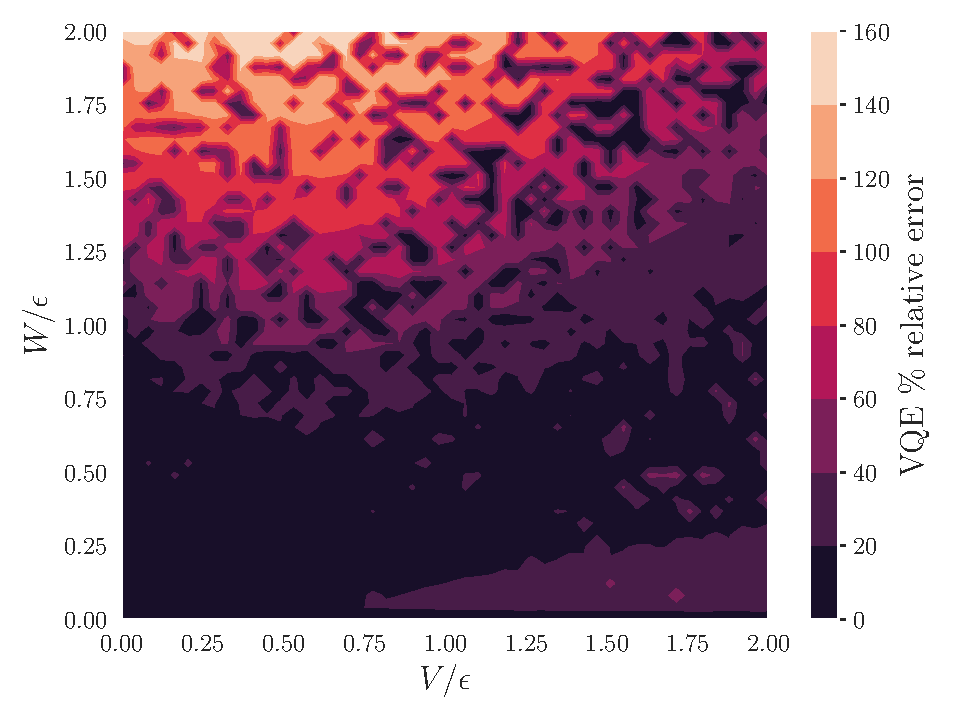
\includegraphics[width=\linewidth]{figs/50pts_vw_grid.pdf}
    \caption{Ground state values for the Lipkin model for $N=4$ particles with $W = 0$ as a function of $V/\epsilon$. Calculations were done using exact diagonalization, VQE, in addition to closed form HF and RPA expressions.}
    \label[fig]{fig:res:lipkin_N4_vw_grid}
\end{figure}
